\chapter{Current state}
\label{ch:currentState}

\section{A brief introduction into discrete two-dimensional convolution}

The model that is used for this project is from the family of convolutional neural networks or CNNs. These are models that are especially useful to perform operations on digital images. CNNs contain at least one convolutional layer that computes a mathematical operation that is called discrete convolution. Discrete convolution operation has been proved useful when applied on digital images to detect structural features like edges and corners. When applying discrete convolution to an image (a two dimensional array of values), a filter with a given two dimensional kernel is used to perform convolution on the image. With the given kernel, a segment that has the same size as the kernel is taken from the input image and an elementwise multiplication between these two matrices is performed. The sum of the results gets written in the output (also called feature map). As most kernels are much smaller than the input image, this inevitable results in smaller feature maps than input images, especially after applying convolution to the same image multiple times. To solve this problem, one can add a padding (increase the image size by adding specific values). An example of a two dimensional convolution operation with padding is shown here:

\begin{figure}[H]
	\center{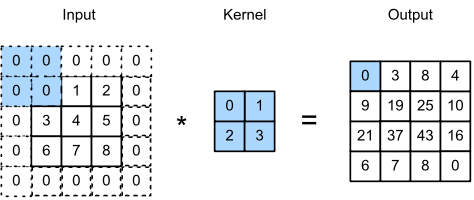
\includegraphics[width=\textwidth]
	{img/2d-convolution.png}}
	\caption{\label{fig:convolution} Example of a two dimensional convolution operation with padding}
\end{figure}

After the convolution is computed for a specific segment, the kernel shifts further some steps in the image array, called stride. There exists a lot of different kernels for different purposes. To detect edges and corners there exist specific kernels especially for that kind of task. For example if one wants to detect vertical edges, a kernel like the following can be used:
$P_y = \begin{pmatrix}-1 & -1 & -1 \\\ 0 & 0 & 0 \\\ 1 & 1 & 1\end{pmatrix}$, \vspace{0.5cm} to detect diagonal edges, one can use a kernel like the following:
$S_d = \begin{pmatrix}-0 & -1 & -2 \\\ 1 & 0 & -1 \\\ 2 & 1 & 0\end{pmatrix}$ \vspace{0.5cm}

It is also possible to learn the optimal kernel in the process of neural network training.

\section{About convolutional neural networks}

The advantage of CNNs compared to traditional multi layer perceptrons (MLPs) is that discrete convolutional operation is translational invariant. This means it is irrelevant where in a given image a specific object is located: The model will not learn the position of the specific object. Another huge advantage of CNNs over MLPs is that CNNs usually have sparse interactions. This means that it is possible to yield a good performance even if some adjacent layers are not fully connected with each other. Another way to speed up the training process is to use parameter sharing: Some weigths will be used at multiple places at the same time. These two techniques, sparse interactions and parameter sharing does make it possible to train very deep convolutional neural networks in a feasible amount of time.

It is important to note that applying discrete convolution on digital images, only primitive features can be extracted. But by combining convolutional layers with other layer types, it is possible to extract much more complex features that can be used to classify objects as humans or animals or vehicles and so on.

Another important kind of layer that is usually employed in CNNs are pooling layers. Also called subsampling or downsampling layers sometimes, they reduce the size of a given image, by computing a statistic metric to summarize multiple values. Some frequently used pooling layers are max- and average-pooling. The advantages of pooling layers are smaller input, parameter reduction and higher invariance to scaling and transformations.

The third important kind of layer is ReLU (rectified linear unit), which computes an activation function used by the neural network. The mere use of this layer is to preprocess the image before the next convolutional operation. This just adjusts the image brightness in a ways that all negative values (values that are darker than the middle grey of an image) got adjusted to middle grey.

The last layer of a CNN contains the number of classes that the network should predict. This layer is usually fully connected to the layer before.

\section{From CNNs to Mask R-CNN}

The very first CNN appeared in the year 1994, it was named LeNet5, after Yann LeCun. This fundamental work was the first network that used convolutional and pooling layers to process images. In a time long before consumer graphic processing units (GPUs), where even CPUs were slow, it was crucial to reduce the number of parameters to a bare minimum (accomplished with sparse connect layers). An image, showing LeNet5 with its different layers and operations in between is shown here:

\begin{figure}[H]
	\center{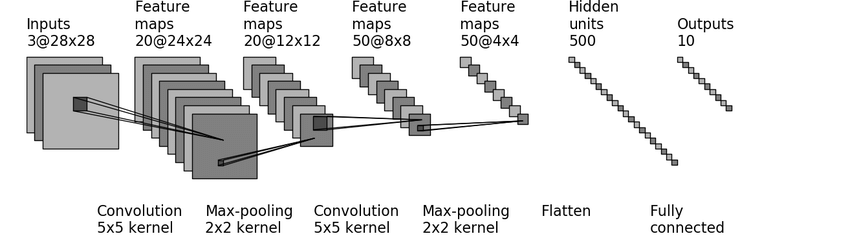
\includegraphics[width=\textwidth]
	{img/lenet5.png}}
	\caption{\label{fig:lenet5} Overview of LeNet5 from the year 1994}
\end{figure}

Starting with AlexNet by Alex Krizhevsky, Ilya Sutskever and Geoffrey Hinton in 2012, CNNs gained significantly performance gains when applied on image classification tasks. AlexNet took the idea of a CNN from LeNet5 and added more layers to the network and was the first to include ReLU layers. It also used dropout techniques to avoid overfitting during the training process. AlexNet was still an image detection or image classification model, trained to label images. This means a single label (class) is given to a whole input image.

ResNet (residual neural network) in 2015 was the first CNN that included residual blocks or identity shortcut connections. These are connections in the network that skip one or more layers and just use the input value as an output (called mathematical identity). This was another step to reduce computation cost and lead to even deeper networks. ResNet is still used today as part of the backbone in a lot of object detection and instance segmentation models.

With R-CNN (regions with CNN features) in 2013, the rise of object detection models began. These researcher asked themselves, how can one use the techniques from CNNs to not only classify an image but to classify multiple objects in that image?  These family of models are capable of labelling multiple objects depicted in the same image with each a bounding box and a class prediction. R-CNN models do that by proposing regions in that potential objects may lie. R-CNN is thus called a two stage model: The first stage scans the image and generates region proposals with the help of a region proposal network (RPN), whereas the second stage uses these regions to extract CNN features from it and to ultimately classify objects in it. For the classification step in the last layer, R-CNN uses a support vector machine (SVM) as a classifier. In the very last step, a regression is used to further tighten the coordinates of the bounding boxes of each object. \cite{R-CNN}

\begin{figure}[H]
	\center{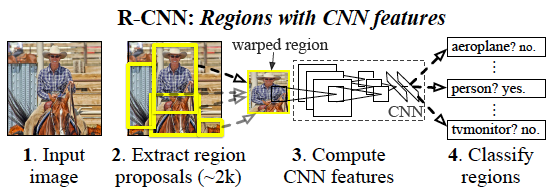
\includegraphics[width=\textwidth]
	{img/r-cnn.png}}
	\caption{\label{fig:r-cnn} Architecture of R-CNN}
\end{figure}

In 2017, the team from Ross Girshick, one of the creators of R-CNN, delivered Fast R-CNN an improved, faster version of it. In R-CNN there are a lot of overlapping region proposals and every computation gets calculated again, even if the regions are very similar to each other. To circumvent this they invented region of interest pooling (RoIPool). RoIPool shares these computation across the regions of an image and can speed up computation time a lot. The other improvement was to put all computations in a single network (compared to R-CNN where for example classification ran in a single network).

Also in 2017 by the team from Ross Girshik, the second iteration of R-CNN got released, called Faster R-CNN. The main improvement was to use just one CNN that produces a single feature map for both region proposal and classification. Features used by both the first and the second stage of the model can be shared to speed up the inference process.

\section{Mask R-CNN}

With Mask R-CNN from 2017 (also by Ross Girshik et. al) it is possible to not only predict the bounding box of an object but also to predict a mask that shows the exact shape of the object (called pixel level segmentation). These models are called instance segmentation models, because they produce a mask for every object in the image. This is accomplished by adding a branch to the Faster R-CNN model that computes a binary mask for a given object in the image. An overview of Mask R-CNN can be seen here:

\begin{figure}[H]
	\center{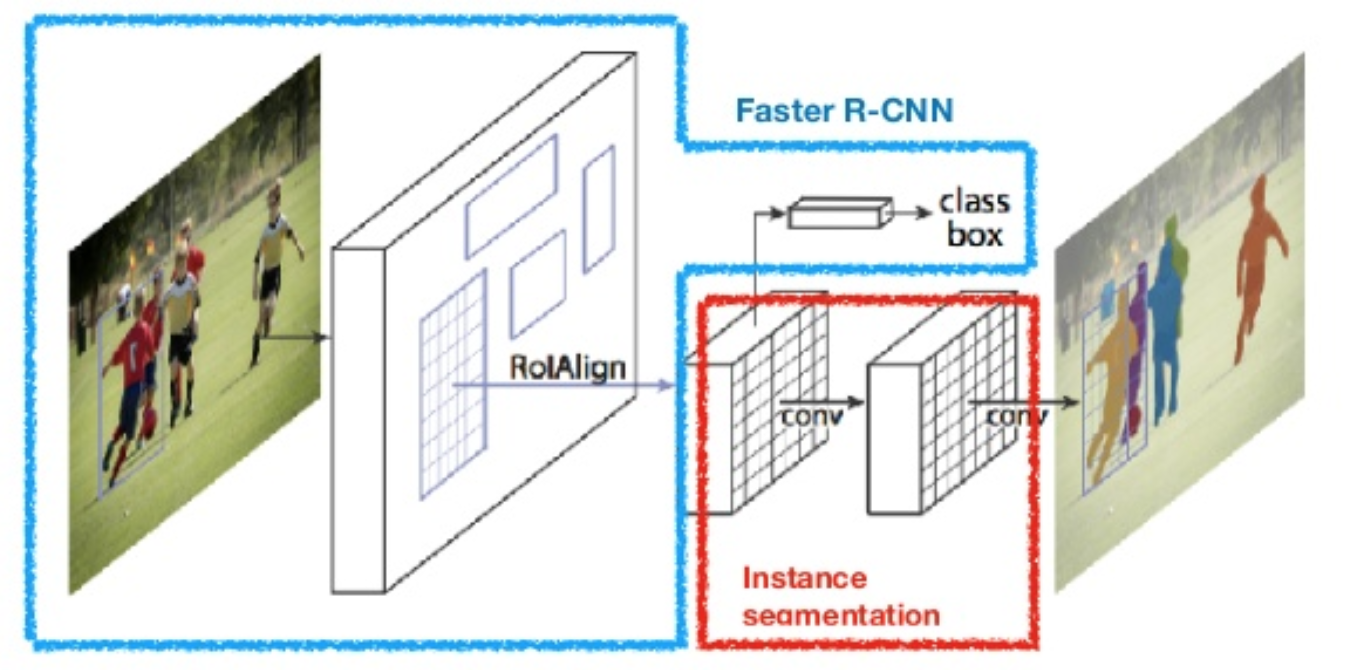
\includegraphics[width=\textwidth]
	{img/maskrcnn2.png}}
	\caption{\label{fig:maskrcnn2} An overview of Mask R-CNN}
\end{figure}

- About feature pyramid networks
- About ResNet101 (backbone)

An overview over the different tasks and approaches and their models  in the field of object recognition can be seen here:

\begin{figure}[!h]
	\center{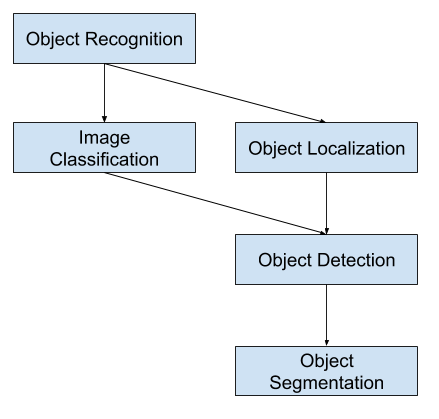
\includegraphics[width=\textwidth]
	{img/object-recognition.png}}
	\caption{\label{fig:object-recognition} Tasks and approaches in object recognition}
\end{figure}

